\documentclass[12pt]{article}

\usepackage[english]{babel}
\usepackage{graphicx}
\usepackage{natbib}
\usepackage{gitinfo2}
\usepackage{amsmath}
\usepackage[T1]{fontenc}
\usepackage[utf8]{inputenc}
\usepackage{authblk}

\renewcommand\Authands{ and }
\newcommand\tab[1][1cm]{\hspace*{#1}}

\title{A simple statistical model describing burnt area through limitations on fire}

\author[1]{Kelley, Douglas \thanks{\textbf{Email:} douglas.i.kelley@gmail.com
                                   \textbf{Web}: douglask3.github.io}}
\author[2, 3]{Bistinas, Ioannis}
\author[4, 5]{Whitley, R}
\author[1]{Marthews, T}

\affil[1]{Centre for Ecology and Hydrology\\
          Maclean Building \\
          Crowmarsh Gifford \\
          Wallingford \\
          Oxfordshire \\
          United Kingdom}

\affil[2]{Vrije Universiteit Amsterdam\\
          Faculty of Earth and Life Sciences \\
          Amsterdam \\
          Netherlands}

\affil[3]{University of Reading\\
          Department of Meteorology\\
          Reading\\
          United Kingdom}

\affil[4]{Suncorp Group \\
          Personal Lines Pricing Research \\
          Sydney \\
          Australia}

\affil[5]{Macquarie University \\
          Department of Biological Sciences \\
          Sydney \\
          Australia}


    

\begin{document}
\maketitle

\begin{abstract}
LimFIRE is a simple statistical model that simulates limitations of fire. Perfect fire conditions are imagined for a location or grid cell, with full fuel coverage, no moisture, saturated igntions and no agricultural or urban fragmentation. In such conditions, 100\% of the land area burns. This is analogous to areas in Northern Australia and parts of the sahel, with areas burning more than once a year. Burnt area is reduced if the location has discontinuous fuel loads  (e.g. desert areas), has fuel to moist to burn (meg. Humid evergreen forests), a lack of ignition (shown to be an influence of inter Annual variability in some parts of the tropical vdv and Southern Australia Bradstock), or human fire suppression (e.g. cropland or urban areas).
\end{abstract}



\begin{center}
    \textbf{git info}

        git url: https://github.com/douglask3/LimFIRE
	
	git revision no: \gitAbbrevHash	

	Last commit author: \gitAuthorName,  \gitAuthorEmail
	
	Branch: \gitReferences	

	Revision Date: \gitAuthorIsoDate 
\end{center}

\section{Introduction}
LimFIRE is a simple statistical model that simulates limitations of fire. Perfect fire conditions are imagined for a location or grid cell, with full fuel coverage, no moisture, saturated igntions and no agricultural or urban fragmentation. In such conditions, 100\% of the land area burns. This is analogous to areas in Northern Australia and parts of the sahel, with areas burning more than once a year. Burnt area is reduced if the location has discontinuous fuel loads  (e.g. desert areas), has fuel to moist to burn (meg. Humid evergreen forests), a lack of ignition (shown to be an influence of inter Annual variability in some parts of the tropical vdv and Southern Australia Bradstock), or human fire suppression (e.g. cropland or urban areas).

\paragraph{Outline}
The remainder of this article is organized as follows.
Section~\ref{previous work} gives account of previous work.
Our new and exciting results are described in Section~\ref{results}.
Finally, Section~\ref{conclusions} gives the conclusions.

\section{Methods}

\subsection{Model}

\begin{equation}
    F=\Pi_{i} (1 - l_i)
\end{equation}

where F is the fractional burnt area, and $l_i$ is the limitation imposed by fuel, moisture, igntions or supresssion.
\newline

or

\begin{equation} 
    F=\Pi_{i} F_i 
\end{equation}

where F is the fractional burnt area, and $F_i$ is the maximum burnt area allowed due to available fuel, moisture, igntions or supresssion. ie, 

\begin{equation}
    F_i = 1 - l_i
\end{equation}

\begin{equation}
    f(x) = (1 + a * e^{-b \cdot x})
\end{equation}

\begin{equation}
\begin{split}
    l_{w} = 1 - f(w) \\
    l_{\omega} = f(\omega) \\
    l_{ig} = 1 - f(ig) \\
    l_{s} = 1- f(s)
\end{split}
\end{equation}


\subsubsection{Fuel ($w$)}

\subsubsection{Moisture ($\omega$)}

\subsubsection{Igntions ($ig$)}

\subsubsection{Supression ($s$)}

\subsection{Analysis}

\subsubsection{Limitation}

\begin{equation}
    \bar{l_{i, X}} = \frac{l_{i, X}}{\sum_{j} l_{j, X}}
\end{equation}

\subsubsection{Sensitivity}

\begin{equation}
    \bar{dl_{i, X}} = \frac{dl_{i, X} \cdot \Pi_{j} l_{j, X}}{l_{i, X}}
\end{equation}

where $dl_{i, X}$ is the gradient of $l_{i, X}$ relative to the maximum possible gradient of $l_{i}$, i.e:

\begin{equation}
    dl_{i, X} = \frac{dl_{i, X} / dx}{dl_{i, l = 0.5} / dx}
\end{equation}

where

\begin{equation}
    \frac{dl_{i}}{dx} 
\end{equation}


\begin{figure}[!ht]
  \centering
    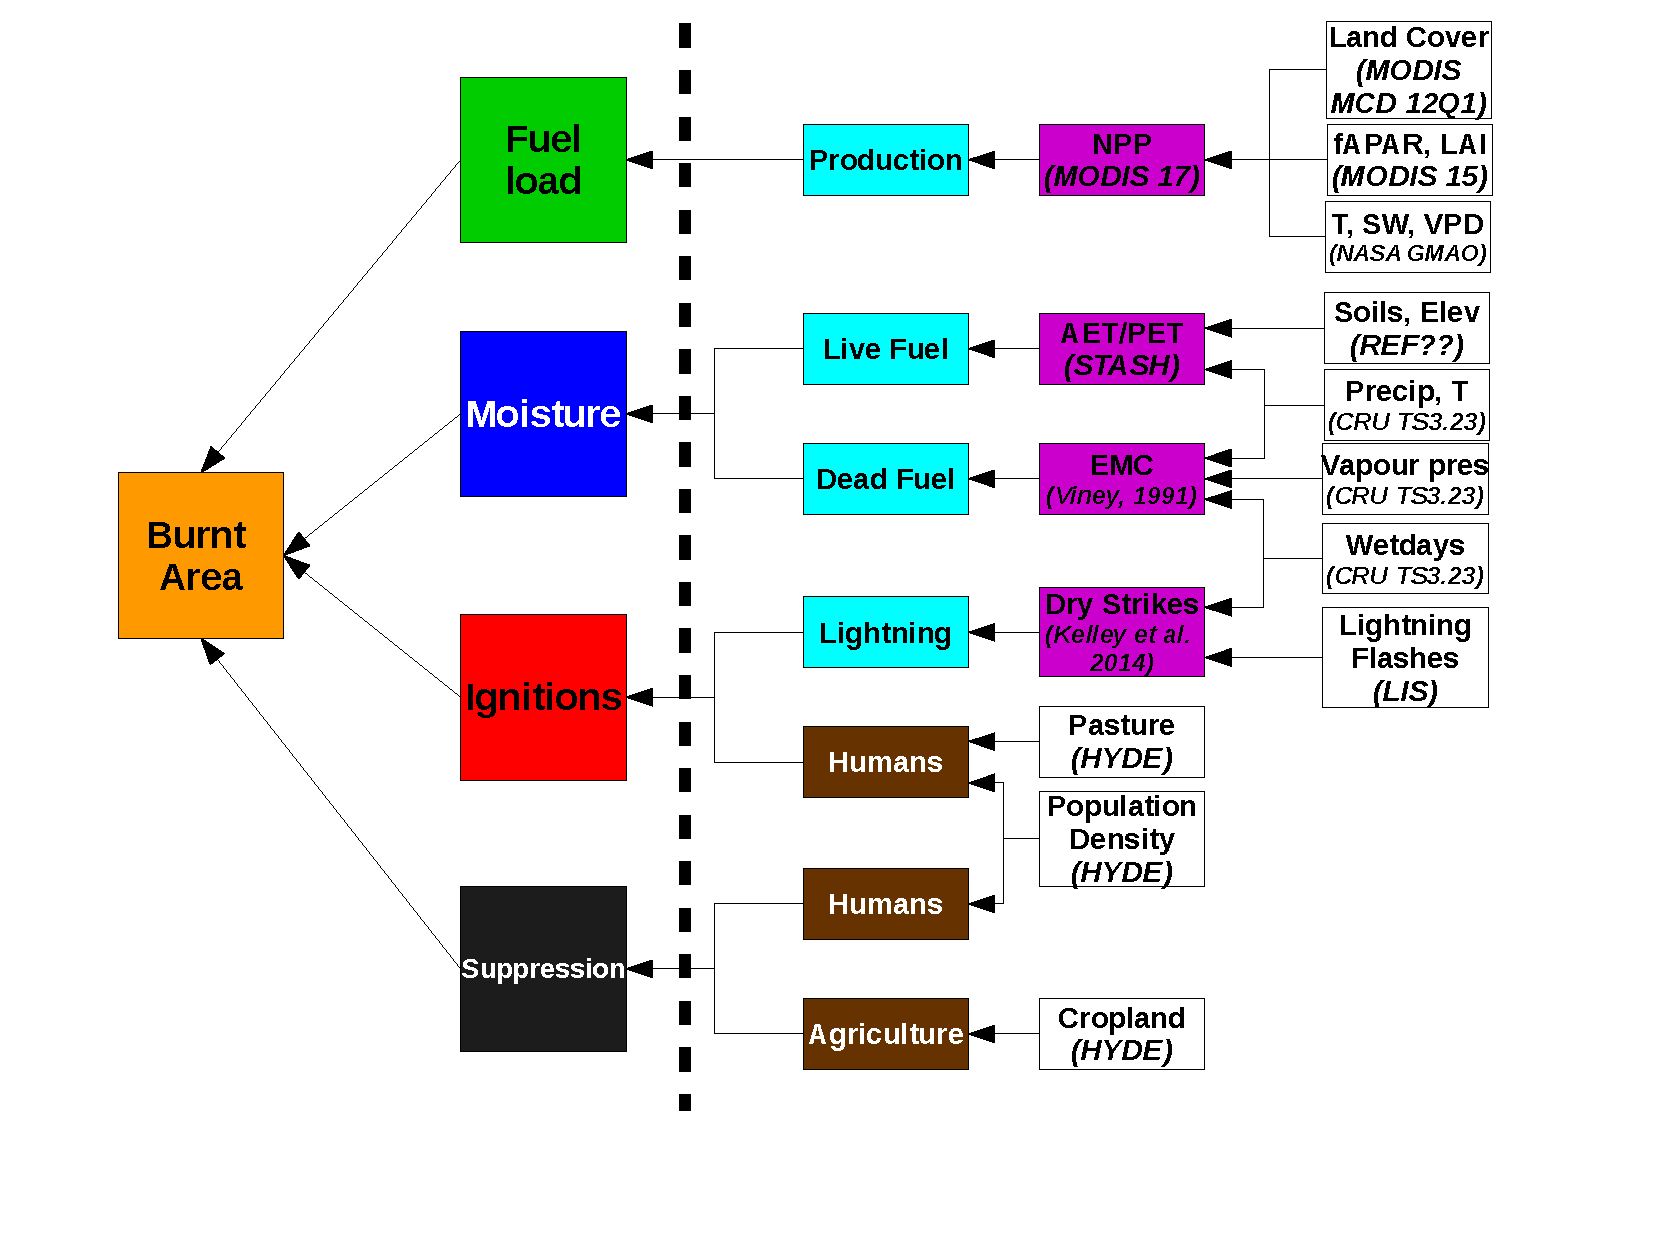
\includegraphics[width=0.67\textwidth]{Model_schematic.pdf}
   
  \caption{Model description.}
\end{figure}


\section{Results}\label{results}
In this section we describe the results.

\subsection{Benchmarking}

\begin{figure}[!ht]
  \centering
    \includegraphics[width=0.67\textwidth]{../figs/gfedComparison.png}
   
  \caption{Benchmark comparisons against GFED4s \citep{Giglio2013}.}
\end{figure}

\subsection{Limitations}

\begin{figure}[!ht]
  \centering
    \includegraphics[width=0.67\textwidth]{../figs/limitation_lines.png}
   
  \caption{Limitation covers.}
\end{figure}

\subsection{Sensitivity}

\begin{figure}[!ht]
  \centering
    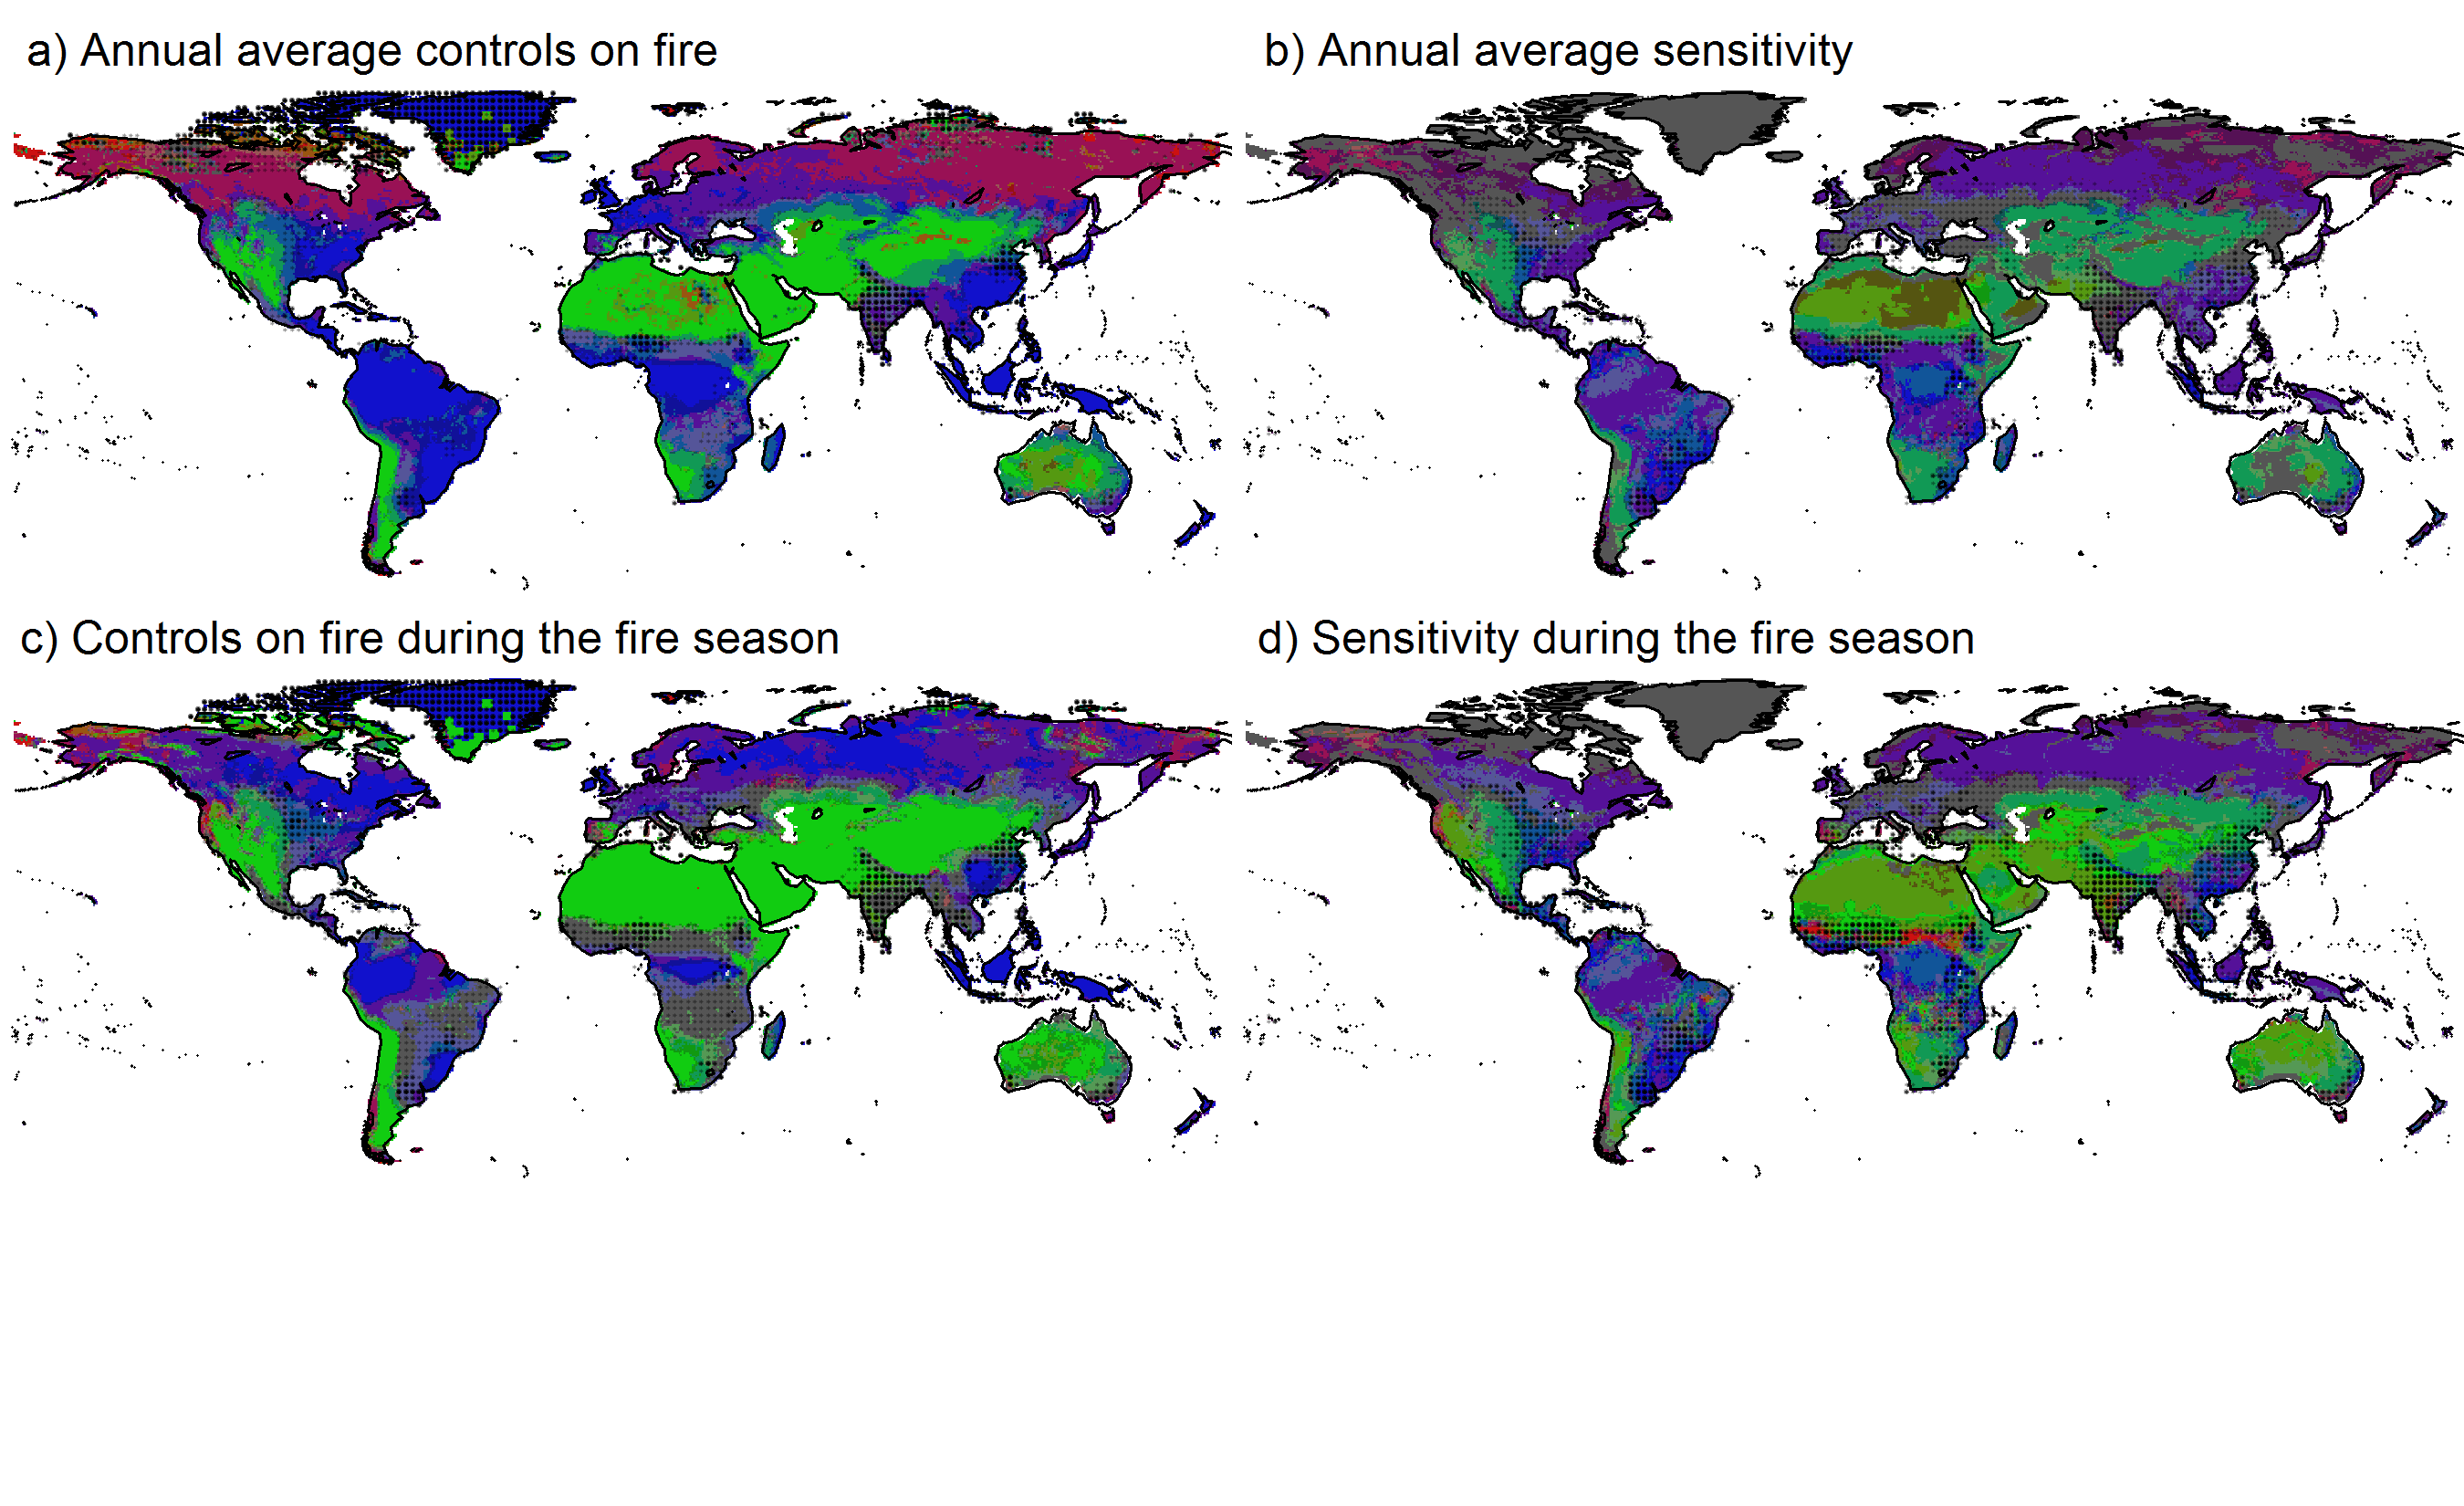
\includegraphics[width=0.67\textwidth]{../figs/limitation_map.png}
   
  \caption{Limitation and sensitivity.}
\end{figure}

\section{Conclusions}\label{conclusions}

\section{Papers and Applications}

\subsection{What limits fire, where and when: sensitivity of burnt area to different controls}

\subsubsection{Abstract}
Global fire models typically describe fire as a consequence of fuel load, moisture, natural and anthropogenic
ignitions, and land use suppression. A lack of information on the temporal and spatial distribution of these
controls has meant that their simulated effects on predicting burnt area are largely untested. Despite this,
there is a pervasive assumption that burnt area is proportional to the number of ignitions, with many models
predicting significant increases in burnt area with human fire starts.


Here, we map the limitation and sensitivity of burnt area to each control using a simple framework whereby
limitations are imposed by: fuel discontinuity; fuel moisture and atmospheric drying potential; lightning and
human ignitions; and land use. Limitations are described from remote sensed and meteorological
observations and optimized against Global Fire Emissions Database (GFED4s) burnt area observations.
Fuel moisture is shown to be the main limitation of fire over much of the world, (44\% annual average and
36\% during local dry seasons), particularly in the humid forests and cold, slow drying boreal areas. Fuel
discontinuity is the next limitation (25\% annually and 23\% in the dry season), especially in deserts and dry
season grasslands. This is followed by land use change (18\% annually, 21\% dry season) and then ignitions
(13\% annually, 19\% dry season), which is only a significant limiting factor in dry season savanna, where
rapid drying of fuel built up during the wet season removes all other natural limitations. In these areas,
changes in burnt area are actually more sensitive to other controls, typically land use.


This study contradicts the way basic processes are represented in many global fire models. As ignitions only
impact burnt area over a limited geographic extent, better representation of controls imposed by fuel loads
and moisture is vital. Human ignitions only contribute to a small increase in global burnt area (2\%), which is
offset by the dramatic impact of suppression through anthropogenic land cover changes. The assumption
that humans cause burnt area over much of the world is therefore clearly incorrect, and adequate simulation
of suppression through land use should become a priority. This result also has implications when considering
ecosystem services of agricultural land and fire management policies.

\pagebreak
x
\pagebreak
\subsection{Anthropagenic regime shifts}
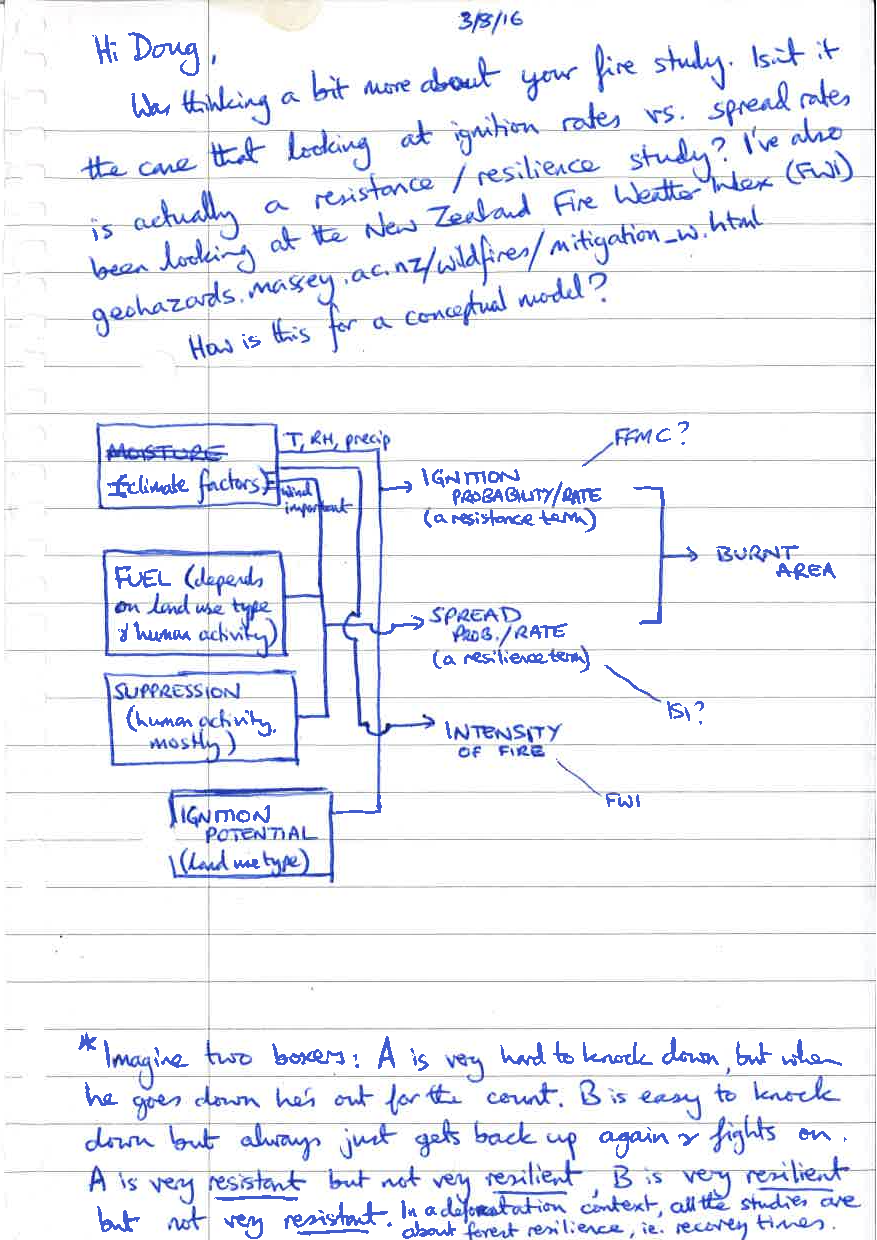
\includegraphics[width=0.99\textwidth]{tobys_notes.pdf}


\bibliographystyle{abbrv}
\bibliography{Model_description}

\end{document}
This is never printed
